\documentclass[english,serif,mathserif]{beamer}
\usetheme[formal,deutsch]{s3it}

\usepackage{graphicx}
\usepackage[T1]{fontenc}
\usepackage[latin9]{inputenc}
\usepackage{babel}
\usepackage{color}

\begin{document}

%% Optional Argument in [Brackets]: Short Title for Footline
\title[Short Title]{MySQL and RabbitMQ} 
\subtitle{Or: OpenStack's core support softwares} 

\author{Tyanko Aleksiev \texttt{<tyanko.aleksiev@s3it.uzh.ch>}}

\date{\today}

\maketitle

% chapter division
\begin{frame}{MySQL's role inside OpenStack}

\textit{MySQL} database assumes a core role in the set of 
support softwares inside OpenStack and is mainly used:

\begin{itemize}
\item for storing the state of the OpenStack cluster (VMs, users, volumes, tokens, etc), 
\item in the workflow of handling new requests (starting a new instance, creating a volume, etc).
\end{itemize}

Alternative of MySQL inside OpenStack is MariaDB.

\end{frame}

\begin{frame}{RabbitMQ's role inside OpenStack}

The \textit{RabbitMQ} messaging system is the second core
support software inside OpenStack and is mainly used:

\begin{itemize}
\item in the process of communication between the different stack components, 
\item in tight collaboration with MySQL in the workflow of handling new requests.
\end{itemize} 

Alternatives of RabbitMQ inside OpenStack are Qpid and ZeroMQ.

\end{frame}
\begin{frame}{MySQL \& RabbitMQ interaction 1/2}

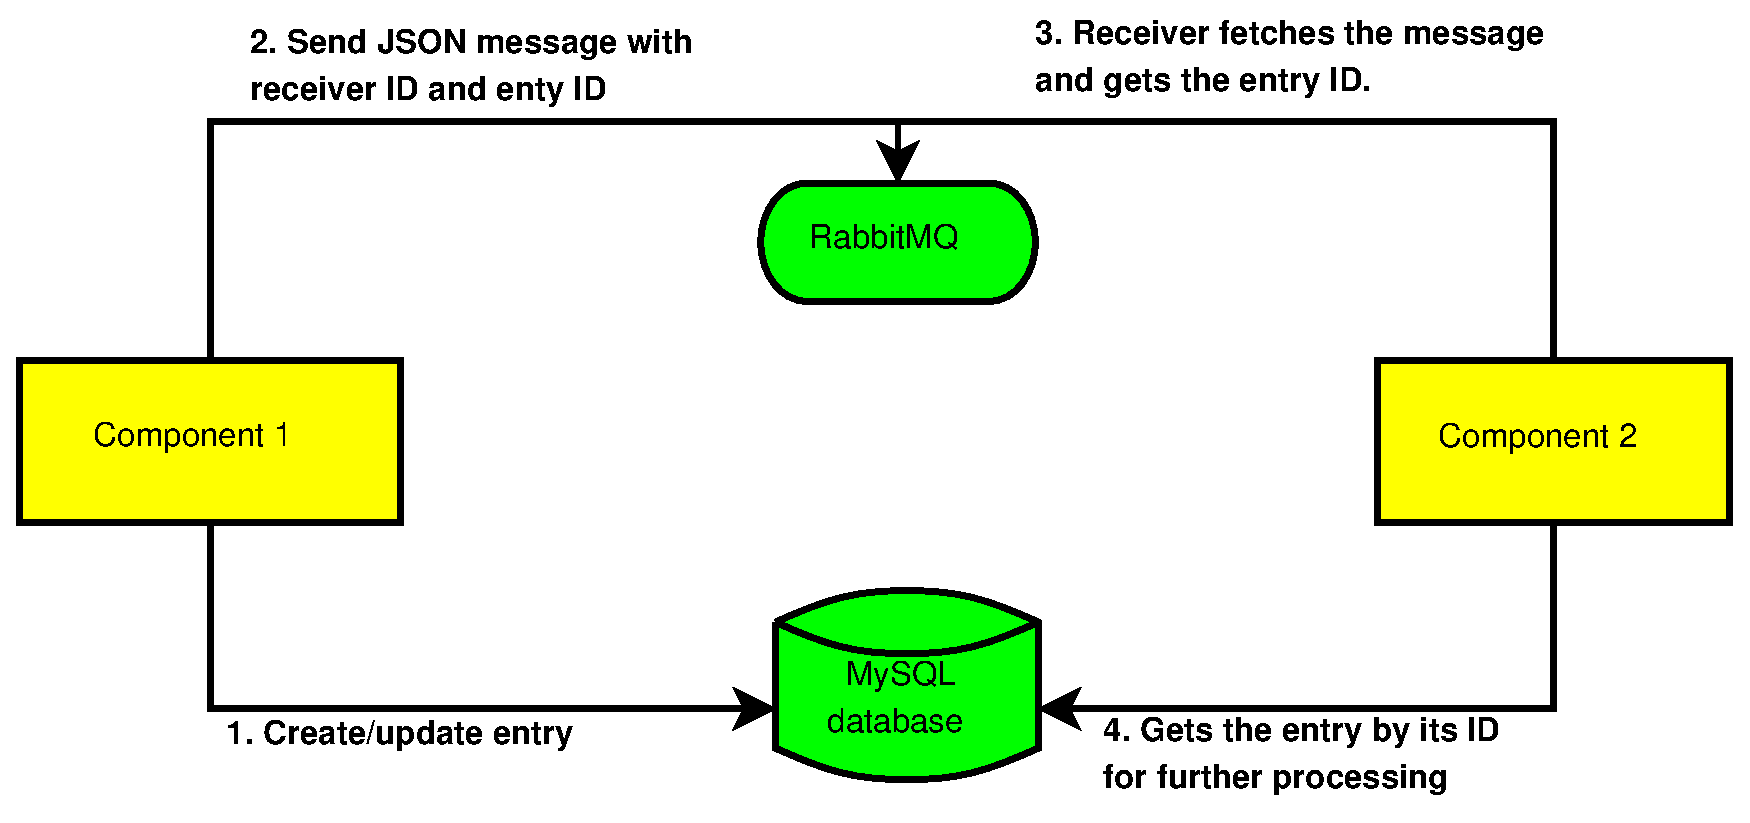
\includegraphics[scale=0.37]{db-rabbitmq.eps}

\end{frame}
\begin{frame}{MySQL \& RabbitMQ interaction 2/2}

Example: provisioning of a new instance

\begin{itemize}
\item a client sends a POST request to nova-api for a VM provisioning,
\item nova-api writes an entry in the DB,
\item nova-api posts then a JSON message in RabbitMQ queue (the message is for nova-scheduler),
\item nova-scheduler reads the JSON message from RabbitMQ queue,
\item nova-scheduler then examines the overall cluster situation from the DB,
\item nova-scheduler posts a JSON message in RabbitMQ saying which compute host should start the VM,
\item nova-compute gathers then the info from the RabbitMQ and from the DB and proceeds with the VM provisioning.
\end{itemize}

\end{frame}



\begin{frame}{MySQL High Availabiltiy}

MySQL is one of the most critical components in the OpenStack installation because 
it contains the state of the whole Stack.

\vspace{5 mm}

Thus, the HA of MySQL becomes critical. The recommended way to do that is by using DRBD and Pacemaker 
even if the alternative method, by using MySQL and Galera, should take over in the near future.

\vspace{5 mm}

Refer to {\color{blue}\href{http://docs.openstack.org/high-availability-guide/content/s-mysql.html}{this}} 
link for more details and info on DRBD and Pacemaker configuration.

\end{frame}

\begin{frame}{RabbitMQ High Availabiltiy}

RabbitMQ can be configured in HA to prevent communication failure between the OpenStack components.

\vspace{5 mm}

This can be achieved again, like with MySQL, by using DRBD and Pacemaker even if the alternative
method, by using two active-active mirrored servers is also becoming important. 

\vspace{5 mm}

Refer to {\color{blue}\href{http://docs.openstack.org/high-availability-guide/content/s-rabbitmq.html}{this}} 
link for more details and info on DRBD and Pacemaker configuration.

\end{frame}

\begin{frame}{Notes and Remarks}

\begin{itemize}
\item Installation of MySQL and RabbitMQ is really straight forward
and requires limited intervention. 
\item Configuration of RabbitMQ is limited to changing the default password.
      \begin{itemize}
          \item Conf. file is \texttt{/etc/rabbitmq/rabbitmq-env.conf}
          \item Logs directory is: \texttt{/var/log/rabbitmq} 
      \end{itemize} 
\item Configuration of MySQL requires a little bit more than RabbitMQ.
      \begin{itemize}
        \item Conf. file is: \texttt{/etc/mysql/my.cnf}
        \item Logs directory is: \texttt{/var/log/mysql}
      \end{itemize}
\item We will see everything in more detail during the tutorial.
\end{itemize}

\end{frame}

\end{document}

%%% Local Variables:
%%% mode: latex
%%% TeX-master: t
%%% End:
